\documentclass{article}\usepackage{graphicx, color}
%% maxwidth is the original width if it is less than linewidth
%% otherwise use linewidth (to make sure the graphics do not exceed the margin)
\makeatletter
\def\maxwidth{ %
  \ifdim\Gin@nat@width>\linewidth
    \linewidth
  \else
    \Gin@nat@width
  \fi
}
\makeatother

\definecolor{fgcolor}{rgb}{0.2, 0.2, 0.2}
\newcommand{\hlnumber}[1]{\textcolor[rgb]{0,0,0}{#1}}%
\newcommand{\hlfunctioncall}[1]{\textcolor[rgb]{0.501960784313725,0,0.329411764705882}{\textbf{#1}}}%
\newcommand{\hlstring}[1]{\textcolor[rgb]{0.6,0.6,1}{#1}}%
\newcommand{\hlkeyword}[1]{\textcolor[rgb]{0,0,0}{\textbf{#1}}}%
\newcommand{\hlargument}[1]{\textcolor[rgb]{0.690196078431373,0.250980392156863,0.0196078431372549}{#1}}%
\newcommand{\hlcomment}[1]{\textcolor[rgb]{0.180392156862745,0.6,0.341176470588235}{#1}}%
\newcommand{\hlroxygencomment}[1]{\textcolor[rgb]{0.43921568627451,0.47843137254902,0.701960784313725}{#1}}%
\newcommand{\hlformalargs}[1]{\textcolor[rgb]{0.690196078431373,0.250980392156863,0.0196078431372549}{#1}}%
\newcommand{\hleqformalargs}[1]{\textcolor[rgb]{0.690196078431373,0.250980392156863,0.0196078431372549}{#1}}%
\newcommand{\hlassignement}[1]{\textcolor[rgb]{0,0,0}{\textbf{#1}}}%
\newcommand{\hlpackage}[1]{\textcolor[rgb]{0.588235294117647,0.709803921568627,0.145098039215686}{#1}}%
\newcommand{\hlslot}[1]{\textit{#1}}%
\newcommand{\hlsymbol}[1]{\textcolor[rgb]{0,0,0}{#1}}%
\newcommand{\hlprompt}[1]{\textcolor[rgb]{0.2,0.2,0.2}{#1}}%

\usepackage{framed}
\makeatletter
\newenvironment{kframe}{%
 \def\at@end@of@kframe{}%
 \ifinner\ifhmode%
  \def\at@end@of@kframe{\end{minipage}}%
  \begin{minipage}{\columnwidth}%
 \fi\fi%
 \def\FrameCommand##1{\hskip\@totalleftmargin \hskip-\fboxsep
 \colorbox{shadecolor}{##1}\hskip-\fboxsep
     % There is no \\@totalrightmargin, so:
     \hskip-\linewidth \hskip-\@totalleftmargin \hskip\columnwidth}%
 \MakeFramed {\advance\hsize-\width
   \@totalleftmargin\z@ \linewidth\hsize
   \@setminipage}}%
 {\par\unskip\endMakeFramed%
 \at@end@of@kframe}
\makeatother

\definecolor{shadecolor}{rgb}{.97, .97, .97}
\definecolor{messagecolor}{rgb}{0, 0, 0}
\definecolor{warningcolor}{rgb}{1, 0, 1}
\definecolor{errorcolor}{rgb}{1, 0, 0}
\newenvironment{knitrout}{}{} % an empty environment to be redefined in TeX

\usepackage{alltt}
\IfFileExists{upquote.sty}{\usepackage{upquote}}{}

\begin{document}

\begin{knitrout}
\definecolor{shadecolor}{rgb}{0.969, 0.969, 0.969}\color{fgcolor}\begin{kframe}
\begin{alltt}

Dataset <- \hlfunctioncall{read.table}(\hlstring{"/home/josephuses/Documents/UPCATReviewer/Test_Item_Analysis/persubject.csv"}, 
    header = TRUE, sep = \hlstring{","}, na.strings = \hlstring{"NA"}, dec = \hlstring{"."}, strip.white = TRUE)
\hlfunctioncall{cor}(Dataset[, \hlfunctioncall{c}(\hlstring{"Biology"}, \hlstring{"Chemistry"}, \hlstring{"English"}, \hlstring{"Filipino"}, \hlstring{"Geology"}, \hlstring{"Math"}, 
    \hlstring{"Physics"})], use = \hlstring{"complete.obs"})
\end{alltt}
\begin{verbatim}
##            Biology Chemistry English Filipino  Geology     Math Physics
## Biology    1.00000   0.22828 0.06244 -0.15134 -0.03737  0.14653 0.05515
## Chemistry  0.22828   1.00000 0.18091  0.15847  0.08424  0.08339 0.19188
## English    0.06244   0.18091 1.00000  0.42153  0.31011  0.06510 0.11064
## Filipino  -0.15134   0.15847 0.42153  1.00000  0.07110 -0.13895 0.08546
## Geology   -0.03737   0.08424 0.31011  0.07110  1.00000  0.14879 0.21620
## Math       0.14653   0.08339 0.06510 -0.13895  0.14879  1.00000 0.15231
## Physics    0.05515   0.19188 0.11064  0.08546  0.21620  0.15231 1.00000
\end{verbatim}
\begin{alltt}
r = \hlfunctioncall{c}(\hlfunctioncall{t}(\hlfunctioncall{as.matrix}(Dataset)))
f = \hlfunctioncall{c}(\hlstring{"Biology"}, \hlstring{"Chemistry"}, \hlstring{"English"}, \hlstring{"Filipino"}, \hlstring{"Geology"}, \hlstring{"Math"}, \hlstring{"Physics"})
k = 7
n = 78
tm = \hlfunctioncall{gl}(k, 1, n * k, \hlfunctioncall{factor}(f))
av = \hlfunctioncall{aov}(r ~ tm)
\hlfunctioncall{summary}(av)
\end{alltt}
\begin{verbatim}
##              Df Sum Sq Mean Sq F value Pr(>F)    
## tm            6  62721   10454    67.5 <2e-16 ***
## Residuals   539  83445     155                   
## ---
## Signif. codes:  0 '***' 0.001 '**' 0.01 '*' 0.05 '.' 0.1 ' ' 1
\end{verbatim}
\begin{alltt}
\hlfunctioncall{TukeyHSD}(av)
\end{alltt}
\begin{verbatim}
##   Tukey multiple comparisons of means
##     95% family-wise confidence level
## 
## Fit: aov(formula = r ~ tm)
## 
## $tm
##                        diff      lwr       upr  p adj
## Chemistry-Biology   -3.6094  -9.5058   2.28712 0.5408
## English-Biology     -5.8429 -11.7394   0.05353 0.0539
## Filipino-Biology     0.7927  -5.1038   6.68917 0.9997
## Geology-Biology    -22.4547 -28.3512 -16.55826 0.0000
## Math-Biology       -29.2074 -35.1039 -23.31095 0.0000
## Physics-Biology    -12.5838 -18.4803  -6.68736 0.0000
## English-Chemistry   -2.2336  -8.1301   3.66289 0.9216
## Filipino-Chemistry   4.4021  -1.4944  10.29853 0.2921
## Geology-Chemistry  -18.8454 -24.7419 -12.94890 0.0000
## Math-Chemistry     -25.5981 -31.4946 -19.70159 0.0000
## Physics-Chemistry   -8.9745 -14.8710  -3.07801 0.0002
## Filipino-English     6.6356   0.7392  12.53212 0.0160
## Geology-English    -16.6118 -22.5083 -10.71531 0.0000
## Math-English       -23.3645 -29.2610 -17.46801 0.0000
## Physics-English     -6.7409 -12.6374  -0.84442 0.0135
## Geology-Filipino   -23.2474 -29.1439 -17.35095 0.0000
## Math-Filipino      -30.0001 -35.8966 -24.10365 0.0000
## Physics-Filipino   -13.3765 -19.2730  -7.48006 0.0000
## Math-Geology        -6.7527 -12.6492  -0.85621 0.0132
## Physics-Geology      9.8709   3.9744  15.76738 0.0000
## Physics-Math        16.6236  10.7271  22.52007 0.0000
\end{verbatim}
\begin{alltt}
\hlfunctioncall{summary}(Dataset)
\end{alltt}
\begin{verbatim}
##     English        Filipino       Geology        Physics     
##  Min.   : 0.0   Min.   : 0.0   Min.   :20.0   Min.   : 3.33  
##  1st Qu.:46.1   1st Qu.:42.1   1st Qu.:37.1   1st Qu.:46.67  
##  Median :50.8   Median :48.3   Median :42.9   Median :55.00  
##  Mean   :51.3   Mean   :47.7   Mean   :45.5   Mean   :52.09  
##  3rd Qu.:58.5   3rd Qu.:55.0   3rd Qu.:51.4   3rd Qu.:60.00  
##  Max.   :87.7   Max.   :80.0   Max.   :77.1   Max.   :73.33  
##    Chemistry       Biology          Math     
##  Min.   : 0.0   Min.   : 0.0   Min.   :11.7  
##  1st Qu.:23.3   1st Qu.:13.3   1st Qu.:32.1  
##  Median :30.0   Median :23.3   Median :38.3  
##  Mean   :28.9   Mean   :22.1   Mean   :38.7  
##  3rd Qu.:35.8   3rd Qu.:33.3   3rd Qu.:44.6  
##  Max.   :53.3   Max.   :60.0   Max.   :65.0
\end{verbatim}
\begin{alltt}
\hlfunctioncall{var}(Dataset)
\end{alltt}
\begin{verbatim}
##           English Filipino Geology Physics Chemistry Biology    Math
## English   197.384    76.13  53.460   19.37    24.533  12.924   9.371
## Filipino   76.129   165.25  11.215   13.69    19.663 -28.662 -18.300
## Geology    53.460    11.21 150.565   33.06     9.977  -6.755  18.705
## Physics    19.371    13.69  33.059  155.29    23.081  10.126  19.446
## Chemistry  24.533    19.66   9.977   23.08    93.169  32.465   8.246
## Biology    12.924   -28.66  -6.755   10.13    32.465 217.069  22.118
## Math        9.371   -18.30  18.705   19.45     8.246  22.118 104.968
\end{verbatim}
\begin{alltt}
\hlfunctioncall{sd}(Dataset)
\end{alltt}


{\ttfamily\noindent\color{warningcolor}{\#\# Warning: sd(<data.frame>) is deprecated.\\\#\#\ \ Use sapply(*, sd) instead.}}\begin{verbatim}
##   English  Filipino   Geology   Physics Chemistry   Biology      Math 
##    14.049    12.855    12.271    12.462     9.652    14.733    10.245
\end{verbatim}
\begin{alltt}
\hlfunctioncall{boxplot}(Dataset)
\end{alltt}
\end{kframe}
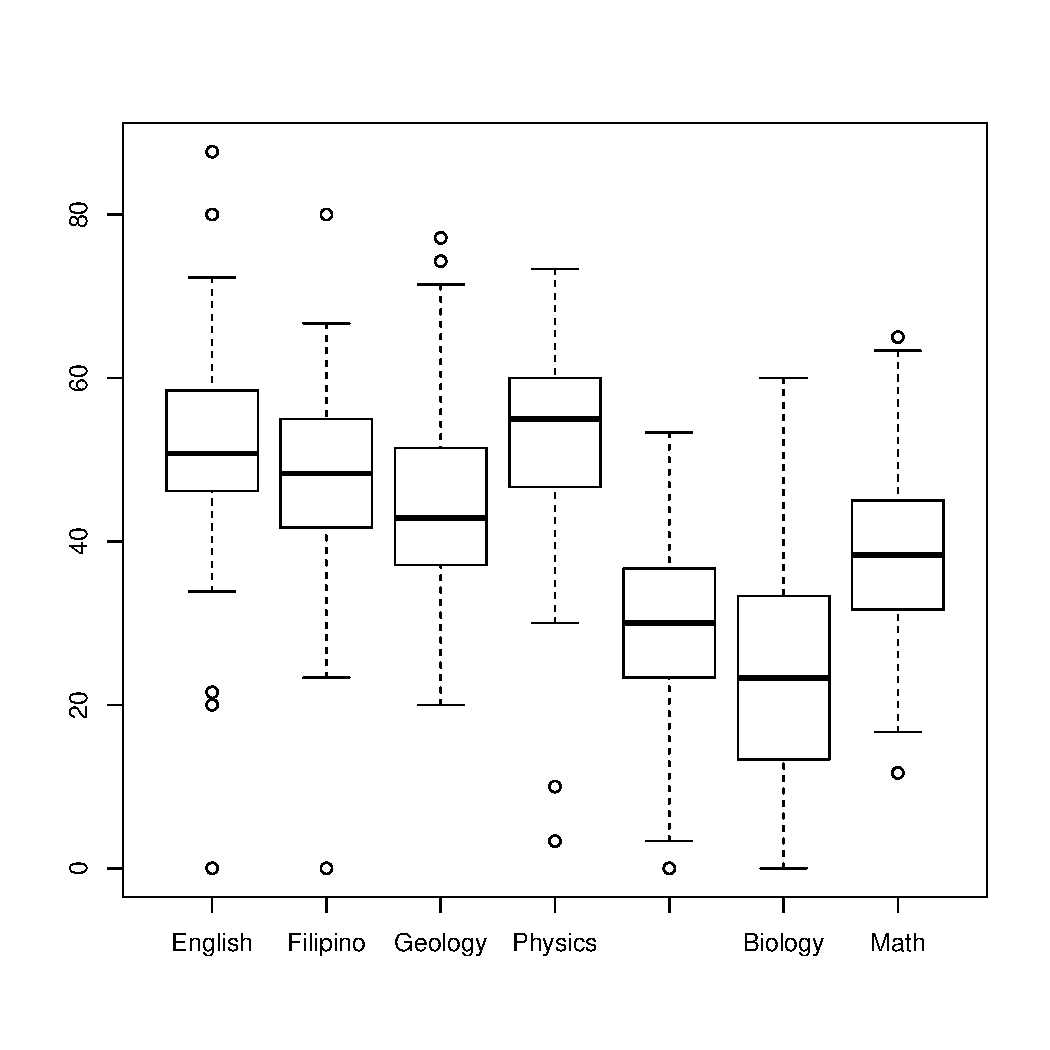
\includegraphics[width=\maxwidth]{figure/wehehehe} 

\end{knitrout}



\end{document}
